% curves.tex

A continuous plane curve is a continuous function $C:[0,1]\to
\RR^2$. $C$ is closed if $C(0) = C(1)$. In order to handle curves
computationally, we approximate them with discrete curves (referred to
as ``curves'' hereafter). We create a curve by choosing a finite
number of sample points $p_0,\dots,p_n\in \RR^2$, where $p_i =
C(t_i)$ for some $0\le t_0 < t_1 < \ldots < t_n \le 1$. A curve is
closed if $p_0 = p_n$.

We can concatenate open curves $C$ and $D$ if the last point of $C$ is
the first point of $D$. We will denote this curve by $CD$. 

We will denote an oriented line segment going from point $p$ to point
$q$ by $\ell_{p,q}$. A curve will then have the form
$$ \ell_{p_0,p_1} \ell_{p_1,p_2}\cdots \ell_{p_{n-1},p_n},$$ and
$p_0$ will be equal to $p_n$ iff the curve is closed. For a closed
curve, this sequence is circular, and we consider any cyclic
permutation of the line segments to be the same curve.

We will denote the length of a curve in segments by $|C|$. A curve $C$
will have $|C|+1$ sample points (counting $p_0 = p_n$ doubly if $C$ is
closed). We will denote the $i$-th sample point of $C$ by $C[i]$,
where $i$ ranges from $0$ to $|C|$.


\subsection{Discretizing for Efficiency}

Our inference and learning algorithms run in time that depends on the
number of sample points in a curve. In particular, parsing takes time
that is cubic in the number of sample points. We can therefore vastly
speed up inference and learning by working with subsampled curves. In
this section, we describe an algorithm that approximates the shape of
a curve with another, coarser curve. 

Let $C$ be a curve with $N$ points. We wish to produce a curve $C'$
such that (a) $C'$ approximates the shape of $C$, (b) $|C'| \approx
L$, and (c) $C'$ is sampled relatively uniformly from $C$. We do this
by minimizing the objective function \eqref{eq:subsample-obj}. The first
term measures the total deviation between $C$ and $C'$, and the second
term rewards relatively uniform sampling at the correct rate.
\begin{equation}
\argmin_{ \{n_i \} } \sum_i \sum_{j=0}^{\lambda_i} \left\| p_{n_i+j} -
  \left( \frac{\lambda_i - j}{\lambda_i} p_{n_i} + \frac{j}{\lambda_i}
    p_{n_{i+1}} \right) \right\|^2 + \alpha \sum_i (\lambda_i -
\widehat{\lambda})^2,\label{eq:subsample-obj}
\end{equation}
where $\lambda_i$ is the length of the $i$-th
segment and $\widehat{\lambda} = N/L$ is the ``ideal'' segment
length. If $C$ is closed, then $p_{n_i + j}$ wraps around: $p_{n_i +
  j} = p_{n_i+j \mod N}$ . This minimization can be done with a
straightforward dynamic program. The results of the algorithm can be
seen in Figure \ref{fig-subsample}.
\begin{figure}[h]
\centering
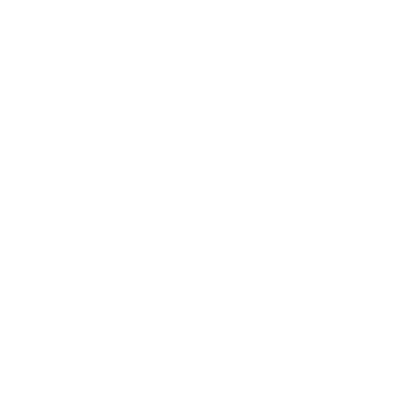
\includegraphics[width=120mm]{images/subsample.png} 
\caption{Subsampled curves. Here $\widehat{\lambda} = 40$}
\label{fig-subsample}
\end{figure}

